Although \corref{etafun_deriv_form} is explicitly about a fixed $\phi$,
it suggests an intriguing result if it is taken to hold for all $\phi$ in some
ball, $\ball_p(\delta) := \{\phi: \norm{\phi}_{\lambda,p} \le \delta \}$.
Specifically, let $q^{-1} + p^{-1} = 1$ and observe that, by Holder's inequality,
%
\begin{align*}
%
\sup_{\phi \in \ball_p(\delta)} \fracat{d \etaopt(\t \phi)}{d \t}{0} ={}&
    \sup_{\phi \in \ball_p(\delta)}
        \int \infl_p(\theta) \phi(\theta) \lambda(d\theta)
\\\le{}&
    \sup_{\phi \in \ball_p(\delta)}
        \left( \int \abs{\infl_p(\theta)}^{1/q} \lambda(d\theta) \right)^q
        \left( \int \abs{\phi(\theta)}^{1/p} \lambda(d\theta)\right)^p
\\={}&
\delta \left( \int \abs{\infl_p(\theta)}^{1/q} \lambda(d\theta) \right)^q,
%
\end{align*}
%
with equality at the ``worst-case'' perturbation
%
\begin{align*}
%
\phi^*(\theta) \propto \abs{\infl_p(\theta)}^{p/q}.
%
\end{align*}
%
The constant of proportionality in the preceding display must be adjusted so
that $\norm{\phi^*(\theta)}_{\lambda,p} = \delta$.  These ``worst-case''
perturbations are the variational Bayes analogues of the corresponding
``worst-case'' for exact Bayesian posteriors in \citet{gustafson:1996:local}.

The worst-case perturbation can be difficult to interpret for several reasons.
First of all, although the ``size'' of a perturbation in $\lp{\lambda,p}$ has
many attractive theoretical properties, it can be hard to have a subjective
opinion about.  Note that the predicted effect of the perturbation is linear in
the $\delta$ in $\ball_p(\delta)$ over which you are taking a supremum; to a
large extent, whether or not a problem is ``robust'' under the perturbation
$\phi^*(\theta)$ will depend on how large $\delta$ is allowed to be, and it can
be difficult to have a strong {\em a priori} opinion about how large $\delta$
should be.  Additionally, the form of $\phi^*(\theta)$ can appear unreasonably
adversarial. Note that the influence function $\psi(\theta)$ is proportional to
the variational posterior $\q(\theta \vert \etaopt)$.  As a result,
$\phi^*(\theta)$ will tend to add and remove a great deal of prior mass
immediately in the vicinity of the posterior mass.  For these reasons,
one might wish to use the influence function more as an informal guide to
selecting and testing perturbations that are likely to be influential.

Whether formally or informally, however, when using a linear approximation to
searching over a in infinite dimensional space, one needs to be concerned about
at least two fundamental properties of your derivative.  First, one must ask
whether the derivative even exists for every $\phi \in \ball_p(\delta)$. More
stringenty, one should also ask whether the derivative forms a uniformly good
approximation to the original function for every $\phi \in \ball_p(\delta)$.
These two properties are formalized in functional analysis by the following
definition.

%%%%%%%%%%%%%%%%%%%%%%%%%%%%%%%%%%%%%%%%%%%%%%%%%%%%%%%%%%%%%%%%%%%%%%%%%%%
%%%%%%%%%%%%%%%%%%%%%%%%%%%%%%%%%%%%%%%%%%%%%%%%%%%%%%%%%%%%%%%%%%%%%%%%%%%
\begin{defn}\deflabel{diffable_classes}
    (\citep[Definition 4.5]{zeidler:2013:functional})
%
Let $B_1$ and $B_2$ denote Banach spaces, and let $\ball_1 \subseteq B_1$ define
an open neighborhood of $\phi_0 \in B_1$.  Fix a function $f: \ball_1
\mapsto B_2$.

The function $f$ is {\em directionally differentiable} (also known as a Gateaux
differentiable) if there exists a bounded linear functional $f^{\mathrm{lin}}:
B_1 \mapsto B_2$ such that the following condition holds for any
$\phi$ with $\norm{\phi - \phi_0} < \infty$:
%
\begin{align*}
%
%\textrm{For any }\phi\textrm{ with }\norm{\phi - \phi_0} < \infty\textrm{, }
\lim_{t \rightarrow 0}
    \frac{f(\phi) - f(\phi_0) -
          f^{\mathrm{lin}}(t (\phi - \phi_0) )
         }{t} \rightarrow 0.
%
\end{align*}
%

Similarly, the function $f$ is {\em boundedly differentiable} (also known as
Fr{\'echet} differentiable) at $\phi_0$ if we can take the limit uniformly in
$\phi$:
%
\begin{align*}
%
\lim_{t \rightarrow 0}
    \sup_{\phi: \norm{\phi - \phi_0} = 1}
    \frac{f(\phi) - f(\phi_0) -
          f^{\mathrm{lin}}(t (\phi - \phi_0))
         }{t} \rightarrow 0.
%
\end{align*}
%
\end{defn}
%%%%%%%%%%%%%%%%%%%%%%%%%%%%%%%%%%%%%%%%%%%%%%%%%%%%%%%%%%%%%%%%%%%%%%%%%%%

Note that we used the same notation $f^{\mathrm{lin}}$ for both derivatives in
\defref{diffable_classes}.  In fact, if a function is Fr{\'e}chet differentiable
then the two derivatives must coincide \citep[Proposition
4.8]{zeidler:2013:functional}, which justifies our presumptuous notation.

In order to motivate our concern, let us consider the following simple example.
It is possible for functions to be directionally but not boundedly
differentiable even in $\mathbb{R}^2$, as the following example demonstrates.

%%%%%%%%%%%%%%%%%%%%%%%%%%%%%%%%%%%%%%%%%%%%%%%%%%%%%%%%%%%%%%%%%%%%%%%%%
%%%%%%%%%%%%%%%%%%%%%%%%%%%%%%%%%%%%%%%%%%%%%%%%%%%%%%%%%%%%%%%%%%%%%%%%%
\begin{ex}\exlabel{r2_pathological}
%
Consider $(x_1, x_2) \in \mathbb{R}^2$ and the polar coordinates $r :=
\sqrt{x_1^2 + x_2^2}$ and $\theta := \arctan(x_2 / x_1)$.  Let $\{\pi k: k \in
\mathbb{Z} \}$ denote integer multiples of $\pi$.  Define
%
\begin{align*}
%
f(r, \theta) := \begin{cases}
    \left(\frac{r}{| \sin \theta |}\right)^2
        & \textrm{when } \theta \notin \{\pi k: k \in \mathbb{Z}\}
        \textrm{ and } r > 0 \\
    0. & \textrm{when } \theta \in \{\pi k: k \in \mathbb{Z}
        \} \textrm{ or }r = 0
%
\end{cases}
%
\end{align*}
%
%%%%%%%%%%%%%%%%%%%%%%%%%%%%%%%%%%%%%%%%%%%%%%%%%%%%%%%%%%%%%%%%%%%%%%%%%
%%%%%%%%%%%%%%%%%%%%%%%%%%%%%%%%%%%%%%%%%%%%%%%%%%%%%%%%%%%%%%%%%%%%%%%%%
\begin{figure}[h!]

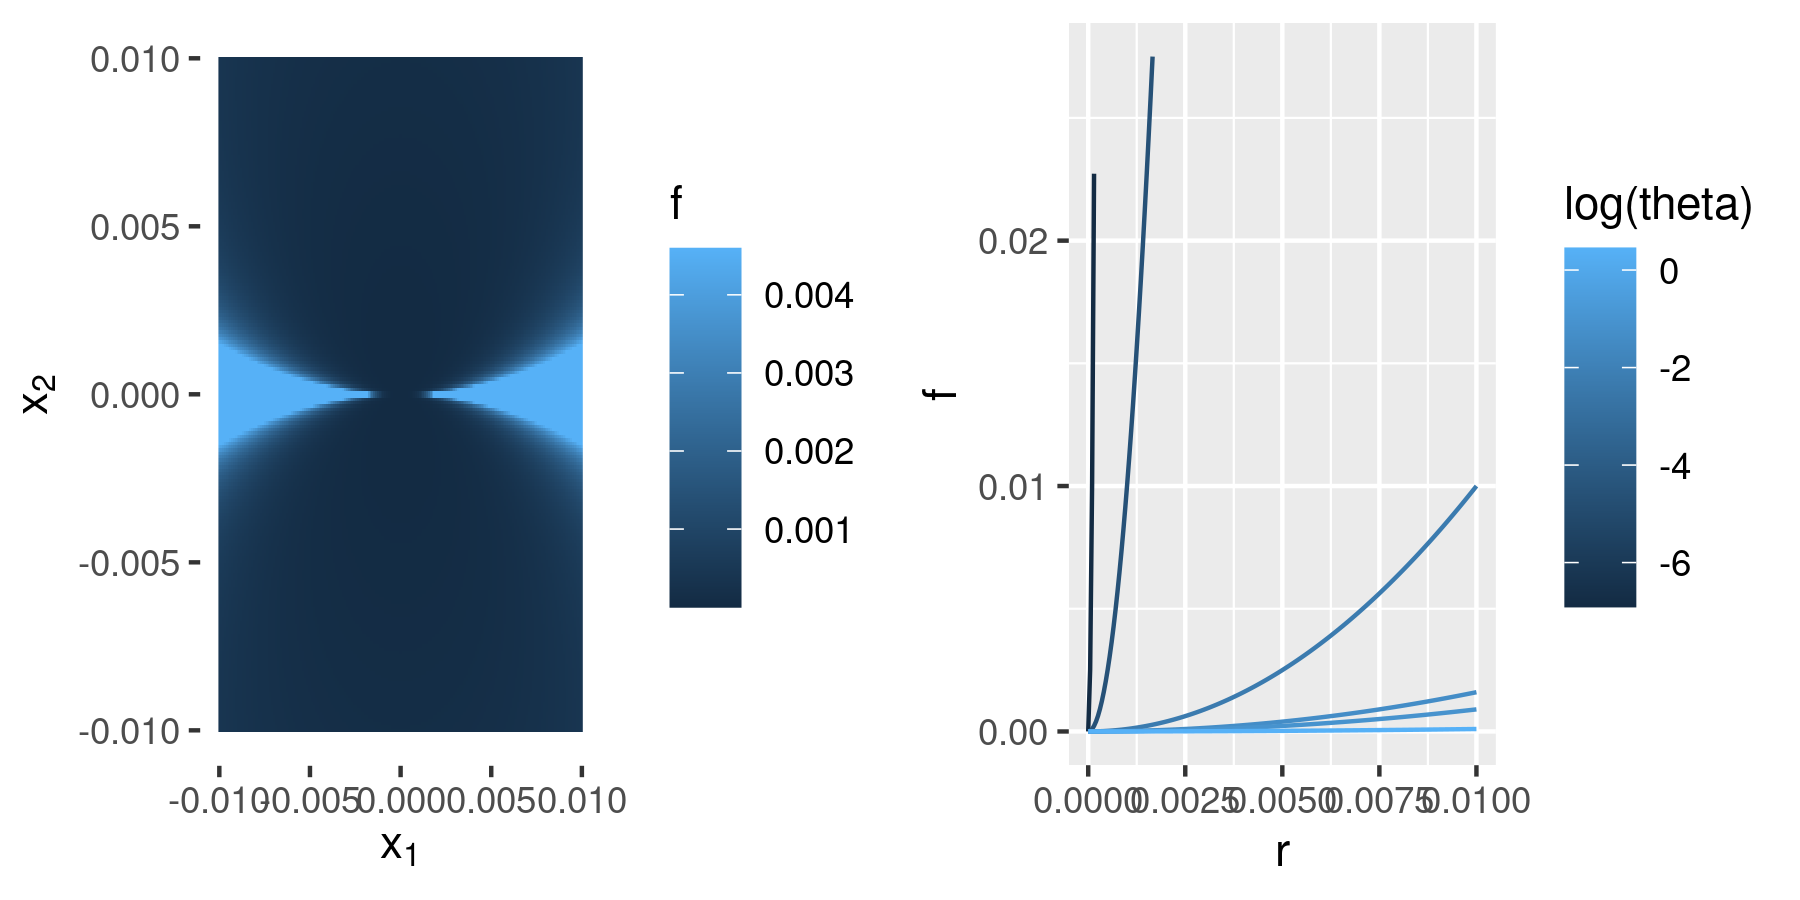
\includegraphics[width=0.980\linewidth,height=0.490\linewidth]{static_images/pathological_r2_example.png}
\caption{A plot of $f(x_1, x_2)$ from \exref{r2_pathological}.}
\figlabel{r2_pathological}
\centering
\end{figure}
%%%%%%%%%%%%%%%%%%%%%%%%%%%%%%%%%%%%%%%%%%%%%%%%%%%%%%%%%%%%%%%%%%%%%%%%%
%
\Figref{r2_pathological} contains a plot of $f(r, \theta)$, both over
$\mathbb{R}^2$ and along paths for particular choices of $\theta$.

We now show that $f$ has a directional derivative in every direction, but is not
Fr{\'e}chet differentiable.  By ordinary calculus, for any $\theta$,
$\fracat{\partial f(r, \theta)}{\partial r}{r=0} = 0$, so the directional
derivatives all exist and are identically $0$.  However, for any $r$, there
exists a $\theta(r)$ such that $r / |\sin(\theta(r))| = 1$.  For such a choice
of $\theta(r)$, the error in the linear approximation is $f(r, \theta(r)) - 0 =
1/2$, which does not go to zero as $r \rightarrow 0$.

\end{ex}
%%%%%%%%%%%%%%%%%%%%%%%%%%%%%%%%%%%%%%%%%%%%%%%%%%%%%%%%%%%%%%%%%%%%%%%%%

Fr{\'e}chet differentiability is only concerned with an infinitesimal
neighborhood.  The function can behave arbitrarily badly in a region just
outside the point at which the derivative is computed and retain Fr{\'e}che
differentiability. In this sense, Fr{\'e}chet differentiability is a desirable
but not sufficient requirement if we are interested in extrapolating using
linear approximations.  We illustrate this point in the

%%%%%%%%%%%%%%%%%%%%%%%%%%%%%%%%%%%%%%%%%%%%%%%%%%%%%%%%%%%%%%%%%%%%%%%%%
%%%%%%%%%%%%%%%%%%%%%%%%%%%%%%%%%%%%%%%%%%%%%%%%%%%%%%%%%%%%%%%%%%%%%%%%%
\begin{ex}\exlabel{r2_pathological_v2}
%
In \exref{r2_pathological} second derivative in a particular direction is given
by $\fracat{\partial^2 f(r, \theta)}{\partial r^2}{r=0} = \frac{1}{2 |\sin
\theta|}$, which can be made arbitrarily large by taking $\theta$ close to $0$
or to $\pi$.  We could modify $f(r, \theta)$ to be Fr{\'e}chet differentiable by
smoothly ``capping'' $1 / |\sin \theta|$ at some arbitrarily large value.
However, the ability to meaningfully extrapolate $f(r, \theta)$ in the direction
of a very large but finite second derivative will still be extremely limited.

In the context of \exref{r2_pathological}, fix some $0 < M < \infty$,
and define
%
\begin{align*}
%
\tilde{f}(r, \theta) := \begin{cases}
    f(r, \theta) & \textrm{when }\frac{1}{\abs{\sin(\theta)}} \le M \\
    0. & \textrm{when }\frac{1}{\abs{\sin(\theta)}} > M.
%
\end{cases}
%
\end{align*}
%
Then $\tilde{f}$ is continuous and Fr{\'e}chet differentiable at $r=0$. In this
case, for any $r$, $\sup_{\theta} r / |\sin(\theta(r))| = r / M$, so  both
$\lim_{r \rightarrow 0} \tilde{f}(r, \theta) \le \lim_{r \rightarrow 0} r^2 /
M^2 = 0$ and $\lim_{r \rightarrow 0} \tilde{f}(r, \theta) / r \le \lim_{r
\rightarrow 0}  r / M^2 = 0$.  (Note that $\tilde{f}$ is continuous only
at $r=0$, not on a ball centered at $0$.)

Despite being Fr{\'e}chet differentiable, the linear approximation may not
extrapolate well to any finite $r$.  In the direction $\theta = \sin^{-1}(1 /
M)$, the error of the linear extrapolation to any $r_0$ is still $\tilde{f}(r,
\theta) - 0 = M r_0^2$. Since Fr{\'e}chet differentiability requires only $M <
\infty$, the extraplation error can be arbitrarily large, even for Fr{\'e}chet
differentiable functions.

\end{ex}
%%%%%%%%%%%%%%%%%%%%%%%%%%%%%%%%%%%%%%%%%%%%%%%%%%%%%%%%%%%%%%%%%%%%%%%%%


\Exref{r2_pathological} is neither Fr{\'e}chet differentiable nor continuous,
whereas \exref{r2_pathological} is both Fr{\'e}chet differentiable and
continuous.  In general, however, Fr{\'e}chet differentiability is stronger than
continuity, in the sense that Fr{\'e}chet differentiability implies continuity,
but continuity does not imply Fr{\'e}chet differentiability \citep[Proposition
4.8 (d)]{zeidler:2013:functional}.  See also \citet[Example
1.9]{averbukh:1967:theory} for a simple example of a function on $\mathbb{R}^2$
that is continuous and directionally differentiable but not Fr{\'e}chet
differentiable.

The sort of pathology exhibited by \exref{r2_pathological, r2_pathological_v2}
requires some care to construct in $\mathbb{R}^2$, but requires some care to
avoid in infinite-dimensional spaces.  We now give an illustrative example in
the $\lp{p}$ spaces.


%%%%%%%%%%%%%%%%%%%%%%%%%%%%%%%%%%%%%%%%%%%%%%%%%%%%%%%%%%%%%%%%%%%%%%%%%
%%%%%%%%%%%%%%%%%%%%%%%%%%%%%%%%%%%%%%%%%%%%%%%%%%%%%%%%%%%%%%%%%%%%%%%%%
\begin{ex}\exlabel{e_log_disocontinuous_v1}
%
Let $\q(\theta)$ and $\p(\theta)$ be densities relative to a continuous measure
$\lambda$.  Let $\gamma \in \lp{\p,p}$ with $1 \le p < \infty$, and define
%
\begin{align*}
%
f(\gamma) = \begin{cases}
\expect{\q(\theta)}{\log\left(1 + \gamma\right)}
    & \textrm{when }\inf_\theta \gamma(\theta) > -1 \\
-\infty & \textrm{otherwise}.
\end{cases}
%
\end{align*}
%
Then $f(\gamma)$ is trivially discontinuous at $\phiz$ since, for any $\gamma$
such that $\inf_\theta \gamma(\theta) = -\infty$,
%
\begin{align*}
%
f(\t \gamma) = -\infty \mathtxt{for any }\t > 0 \mathtxt{but} f(\phiz) = 0.
%
\end{align*}
%
\end{ex}
%%%%%%%%%%%%%%%%%%%%%%%%%%%%%%%%%%%%%%%%%%%%%%%%%%%%%%%%%%%%%%%%%%%%%%%%%

The problem with \exref{e_log_disocontinuous_v1} is not merely with
functions unbounded below, however.

%%%%%%%%%%%%%%%%%%%%%%%%%%%%%%%%%%%%%%%%%%%%%%%%%%%%%%%%%%%%%%%%%%%%%%%%%
%%%%%%%%%%%%%%%%%%%%%%%%%%%%%%%%%%%%%%%%%%%%%%%%%%%%%%%%%%%%%%%%%%%%%%%%%
\begin{ex}\exlabel{e_log_disocontinuous_v2}
%
In the setting of \exref{e_log_disocontinuous_v1}, assume further that, for any
$\epsilon \ge 0$, there exists a set $S_\epsilon$ such that $\p(S_\epsilon) \le
\epsilon$ and $\q(S_\epsilon) \ge \epsilon$.  Define
%
\begin{align*}
%
\tilde{f}(\gamma) = \begin{cases}
    f(\gamma) & \textrm{when }\inf_\theta \gamma(\theta) > -\infty \\
    0 & \textrm{otherwise}.
\end{cases}
%
\end{align*}
%
Now, with $\gamma$ such that $\inf_\theta \gamma(\theta) = -\infty$,
%
\begin{align*}
%
\tilde{f}(\t \gamma) = 0 \mathtxt{for any }\t > 0 \mathtxt{and} f(\phiz) = 0.
%
\end{align*}

However, $\tilde{f}$ is still discontinuous.  For any $\epsilon > 0$, let
$S_\epsilon$ be a set given in the assumption, and for $\delta > 0$, define
%
\begin{align*}
%
\gamma(\theta, \epsilon, \delta) :=
\begin{cases}
    %
    \delta - 1      & \textrm{ for }\theta\in S_\epsilon \\
    0      & \textrm{ for }\theta\notin S_\epsilon.
    %
\end{cases}
%
\end{align*}
%
Then $\gamma(\theta; \epsilon, \delta) \in \lp{\p,p}$ with.  Furthermore,
%
\begin{align*}
%
\norm{\gamma(\cdot;
\epsilon, \delta)}_{\p,p} =
    \left( \int_0^1 \phi(\theta)^p \p(\theta
)\lambda(d\theta)\right)^{1/p} \le{}& \epsilon^{1/p} (\delta - 1)  \mathand\\
%
\abs{\tilde{f}(\gamma(\cdot; \epsilon, \delta)) - \tilde{f}(\phiz)} =
    \expect{\q(\theta)}{\ind{\theta \in S_\epsilon}} \abs{\log(\delta)} \ge{}&
    \epsilon \abs{\log(\delta)}.
%
\end{align*}
%,
Take $\delta(\epsilon) = \exp(-\epsilon)$.  Then, for any sequence $\epsilon_n
\rightarrow 0$,
%
\begin{align*}
%
\abs{\tilde{f}(\phi(\cdot; \epsilon_n, \delta(\epsilon_n))) -
     \tilde{f}(\phiz)} \ge{} 1
\mathtxt{and}
\norm{\gamma(\cdot; \epsilon_n, \delta(\epsilon_n))}_p \rightarrow{} 0.
%
\end{align*}
%
So $\tilde{f}$ is discontinuous on an $\norm{\cdot}_p$ ball containing $\phiz$,
and cannot be Fr{\'e}chet differentiable.
%
\end{ex}
%%%%%%%%%%%%%%%%%%%%%%%%%%%%%%%%%%%%%%%%%%%%%%%%%%%%%%%%%%%%%%%%%%%%%%%%%

Indeed, \exref{e_log_disocontinuous_v2} shows that the KL divergence
cannot be Fr{\'e}chet differentiable for $p < \infty$.

%%%%%%%%%%%%%%%%%%%%%%%%%%%%%%%%%%%%%%%%%%%%%%%%%%%%%%%%%%%%%%%%%%%%%%%%%
%%%%%%%%%%%%%%%%%%%%%%%%%%%%%%%%%%%%%%%%%%%%%%%%%%%%%%%%%%%%%%%%%%%%%%%%%
%
\begin{cor}\corlabel{kl_discontinuous}
%
Assume that $\pbase(\theta)$ and $\q(\theta \vert \eta)$ are defined relative to
the Lebesgue measure, and that $\etaopt$ it a VB optimum.  For $1 \le p <
\infty$, the class of perturbations defined in \defref{prior_nl_pert}, and the
space $\lp{\lambda, p}$, the maps
%
\begin{align*}
%
\phi \mapsto{}& \KL{\etaopt, \phi} \mathand \\
\phi \mapsto{}&
\begin{cases}
    \KL{\etaopt, \phi} & \textrm{when }\inf \phi > -\infty \\
    \KL{\etaopt, \phiz} & \textrm{otherwise}.
\end{cases}
%
\end{align*}
%
are discontinuous at $\phiz$, and so not Fr{\'e}chet differentiable.
%
\begin{proof}
%
For any $\etaopt$, for any set $\S$ with $\expect{\pbase(\theta)}{\ind{S}} > 0$,
$\expect{\q(\theta \vert \etaopt)}{\ind{S}} > 0$ as well, since otherwise
the KL divergence would be infinite and $\etaopt$ cannot be a VB optimum.
Since $\lambda$ is the Lebesgue measure, there exist sets $S_\epsilon$...
TODO a little more work here.

By \eqref{nl_vb_pert_p}, the KL divergence is of the form
%
\begin{align*}
%
\KL{\etaopt, \phi} = \KL{\etaopt, \phiz} +
    p \log\left(1 + \t \frac{\phi(\theta)}{\pbase(\theta)^{1/p}}\right).
%
\end{align*}
%
Define $\gamma(\theta) = \phi(\theta) / \pbase(\theta)^{1/p}$, and note that
$\gamma \in \lp{\pbase, p}$ with $\norm{\gamma}_{\pbase, p} =
\norm{\phi}_{\lambda, p}$.  The results then follow from
\exref{e_log_disocontinuous_v1, e_log_disocontinuous_v2}.
%
\end{proof}
%
\end{cor}
%%%%%%%%%%%%%%%%%%%%%%%%%%%%%%%%%%%%%%%%%%%%%%%%%%%%%%%%%%%%%%%%%%%%%%%%%


Despite \corref{kl_discontinuous}, the directional derivatives exist
as long as $\inf_\theta \phi(\theta) > -\infty$.

%%%%%%%%%%%%%%%%%%%%%%%%%%%%%%%%%%%%%%%%%%%%%%%%%%%%%%%%%%%%%%%%%%%%%%%%%%%%%
%%%%%%%%%%%%%%%%%%%%%%%%%%%%%%%%%%%%%%%%%%%%%%%%%%%%%%%%%%%%%%%%%%%%%%%%%%%%%
\begin{assu}\assulabel{lp_regular}
%
Fix $p$, $\pbase$, and $\lambda$ as in \defref{prior_nl_pert}, and let
$\q(\theta)$ be a density defined relative to $\lambda$.  Let $q$ be the real
number such that $p^{-1} + q^{-1} = 1$.  Fix a function $\psi(\theta): \thetadom
\mapsto \mathbb{R}$ with $\expect{\q(\theta)}{\abs{\psi(\theta)}} < \infty$, and
assume that
%
\begin{align*}
%
\int \abs{\frac{\psi(\theta) \q(\theta)}{\pbase(\theta)}}^q
\pbase(\theta) \lambda(d\theta) < \infty.
%
\end{align*}
%
or, equivalently, that
%
\begin{align*}
%
\int \abs{\frac{\psi(\theta) \q(\theta)}{\pbase(\theta)}}^{q-1}
    \q(\theta) \lambda(d\theta)
< \infty.
%
\end{align*}
%
\end{assu}
%%%%%%%%%%%%%%%%%%%%%%%%%%%%%%%%%%%%%%%%%%%%%%%%%%%%%%%%%%%%%%%%%%%%%%%%%%%%%


%%%%%%%%%%%%%%%%%%%%%%%%%%%%%%%%%%%%%%%%%%%%%%%%%%%%%%%%%%%%%%%%%%%%%%%%%%%%%
%%%%%%%%%%%%%%%%%%%%%%%%%%%%%%%%%%%%%%%%%%%%%%%%%%%%%%%%%%%%%%%%%%%%%%%%%%%%%
\begin{assu}\assulabel{q_regular_lp}
%
For each $\eta$ in an open set $\ball_\eta$, let \assuref{lp_regular} hold with
$\psi(\theta)$ equal to each of the following functions:
%
\begin{align*}
%
& \norm{\lqgrad{\theta, \eta}}_2 \\
& \norm{\lqgrad{\theta, \eta}}^2_2 \\
& \norm{\lqhess{\theta, \eta}}^2.
%
\end{align*}
%
\end{assu}
%%%%%%%%%%%%%%%%%%%%%%%%%%%%%%%%%%%%%%%%%%%%%%%%%%%%%%%%%%%%%%%%%%%%%%%%%%%%%


%%%%%%%%%%%%%%%%%%%%%%%%%%%%%%%%%%%%%%%%%%%%%%%%%%%%%%%%%%%%%%%%%%%%%%%%%%%%%
%%%%%%%%%%%%%%%%%%%%%%%%%%%%%%%%%%%%%%%%%%%%%%%%%%%%%%%%%%%%%%%%%%%%%%%%%%%%%

\begin{thm}\lemlabel{lp_derivative}
%
Fix $\pbase$, $\lambda$, and $1 \le p < \infty$ as in \defref{prior_nl_pert}.
Let $\q(\theta \vert \eta)$ define a class of densities relative to $\lambda$
parameterized by $\eta$ in an open ball $\ball_\eta$ satisfying
\assuref{q_regular_lp}.  Let $\etaopt$ be a variational optimum satisfying
\assuref{kl_opt_ok}.

Then, for each $\phi \in \lp{p}$ with $\norm{\phi}_p \le \infty$ and
$\inf_\theta \phi(\theta) > -\infty$, the function $\t \mapsto \etaopt(\t \phi)$
is differentiable at $\t = 0$ with the derivative given in
\corref{etafun_deriv_form}.
%
\begin{proof}
%
The KL divergence is given by
%
\begin{align*}
%
\KL{\eta, \t} ={}&
    \KL{\eta, 0} +
    \expect{\q(\theta \vert \eta)}
           {\log \left(1 + \t \frac{\phi(\theta)}{\pbase(\theta)^{1/p}} \right)}.
%
\end{align*}
%
Define $\gamma(\theta) := \frac{\phi(\theta)}{\pbase(\theta)^{1/p}}$, and note
that $\norm{\gamma}_{\pbase, p} = \norm{\phi}_{p}$, so $\norm{\gamma}_{\pbase,
p} \le \infty$ and $\inf_\theta \gamma(\theta) > -\infty$.  By
\assuref{q_regular_lp} and \lemref{lp_integral_bound}, we have that that
\assuref{dist_fun_nice} holds with $\psi(\theta, \t) = \log \left(1 + \t
\frac{\phi(\theta)}{\pbase(\theta)^{1/p}}\right)$, and \thmref{etat_deriv}
holds.
%
\end{proof}
%
\end{thm}
%%%%%%%%%%%%%%%%%%%%%%%%%%%%%%%%%%%%%%%%%%%%%%%%%%%%%%%%%%%%%%%%%%%%%%%%%%%%%


The problems are only with priors near zero, which are not possible for
the log perturbation.  Indeed, we have:


%%%%%%%%%%%%%%%%%%%%%%%%%%%%%%%%%%%%%%%%%%%%%%%%%%%%%%%%%%%%%%%%%%%%%%%%%%%%
%%%%%%%%%%%%%%%%%%%%%%%%%%%%%%%%%%%%%%%%%%%%%%%%%%%%%%%%%%%%%%%%%%%%%%%%%%%%
\begin{assu}\assulabel{q_fun_stick_regular}
%
Assume that the variational approximations $\q(\nu \vert \etanuk)$ to the
stick-breaking posteriors satisfy \assuref{dist_fun_nice} with $\eta_0 =
\etaopt$ and with $\psi(\zeta, \t) = 1$.
%
\end{assu}
%%%%%%%%%%%%%%%%%%%%%%%%%%%%%%%%%%%%%%%%%%%%%%%%%%%%%%%%%%%%%%%%%%%%%%%%%%%%


%%%%%%%%%%%%%%%%%%%%%%%%%%%%%%%%%%%%%%%%%%%%%%%%%%%%%%%%%%%%%%%%%%%%%%%%%%%%
%%%%%%%%%%%%%%%%%%%%%%%%%%%%%%%%%%%%%%%%%%%%%%%%%%%%%%%%%%%%%%%%%%%%%%%%%%%%
\begin{thm}\thmlabel{eta_phi_deriv}
%
Let \assuref{kl_opt_ok, q_fun_stick_regular} hold. Then the map $\phi \mapsto
\etaopt(\phi)$ is well-defined and continuously Fr{\'e}chet differentiable in a
neighborhood of $\phiz$ as a map from $\linf$ to $\mathbb{R}^\etadim$,
with the derivative given in \corref{etafun_deriv_form}.

(For a proof, see \appref{proofs} \proofref{eta_phi_deriv}.)
% Furthermore, the derivative at $\phiz$ in the direction $\phi$ is of the form
% %
% \begin{align}
% %
% \fracat{d \etaopt(\phi)}{d\phi}{\phiz} \phi ={}&
%     \int \infl(\nu) \phi(\nu) d\nu \mathtxt{where} \eqlabel{infl_defn}\\
% %
% \infl(\nu) :={}&
% -\left(\fracat{\partial^2 \KL{\eta, \phiz}}
%                 {\partial \eta \partial \eta^T}
%                 {\etaopt}\right)^{-1}
% \left(
%     \sumkm
%     \q(\nu \vert \etaoptnuk) \lqgradbar{\nuk \vert \etanuk}
% \right). \nonumber
% %
% \end{align}
%
%%%%%%%%%%%%%%%%%%%%%%%%%%%%%%%%%%%%%%%%%%%%%%%%%%%%%%%%%%%%%%%%%%%%%%
%%%%%%%%%%%%%%%%%%%%%%%%%%%%%%%%%%%%%%%%%%%%%%%%%%%%%%%%%%%%%%%%%%%%%%

\end{thm}
%
%%%%%%%%%%%%%%%%%%%%%%%%%%%%%%%%%%%%%%%%%%%%%%%%%%%%%%%%%%%%%%%%%%%%%%%%%%%%
